\section{Logistics}
\label{sec:fdsp-tc-log}


Transport is one of the more challenging aspects of the \dword{lbnf} and \dword{dune} endeavor.  
Access to the underground installation area for \dword{lbnf}, \dword{dune}, and \dword{jpo} personnel, as well as  \dword{lbnf} and \dword{dune}  materials and equipment, will be provided by a single shaft, the mile-deep Ross Shaft. 
The shaft is outfitted with a hoist that controls a cage and skips. The cage is used to transport people, equipment and materials, and the skips to bring up muck and transport over-sized equipment and materials.

Due to the enormous cost of the \dword{lbnf}-\dword{cf} contracts and the risk of increased construction costs due to materials supply delays, the scheduling of the shaft must be tightly controlled by \dword{lbnf}-\dword{cf} during construction. Therefore, the \dword{lbnf}-\dword{cf} \dword{cmgc} will coordinate overall usage of the Ross Shaft during this period. The \dword{jpo} will establish a logistics organization (operated under the Fermilab \dword{sdsd}) and lease a warehouse facility within a maximum one-day roundtrip from \dword{surf} by truck to facilitate the flow of  \dword{lbnf} and \dword{dune} non-\dword{cf} materials and equipment to the Ross Headframe. It is expected that the lease of this facility, referred to as the \dword{sdwf}, will include warehouse space, personnel and a \dword{wms} to inventory all incoming materials and equipment. 
%Given the enormous cost of the \dword{lbnf}-\dword{cf} contracts and the costs of inefficiencies in civil construction if material delivery is delayed the scheduling of the shaft must be controlled by \dword{lbnf}-\dword{cf} during construction. Therefore the \dword{lbnf} \dword{cf} \dword{cmgc} will coordinate overall usage of the Ross Shaft during the construction period.
%The \dword{jpo}  will establish a logistics organization (operated under the \dword{fnal} \dword{sdsd}) and lease a warehouse facility within a two-hour drive of  \dword{surf} to facilitate the flow of \dword{dune} and \dword{lbnf} non\dword{cf} material to the Ross Headframe.  It is expected that this facility , referred to as the \dword{sdwf}, will include warehouse space, personnel and a \dword{wms} system for inventory.  
A facility has not yet been selected. 

%%Preferably all \dword{lbnf} and \dword{dune} 
With only specifically managed exceptions, all other materials and equipment will be shipped to the \dword{sdwf}; \dword{cf} material, and likely cryogenics equipment, are exceptions and will ship directly to \dword{surf}. 
The logistics  organization will be responsible for (1) receiving and inventorying all  goods shipped to the \dword{sdwf}, and (2) coordinating with the \dword{cf}-\dword{cmgc}  to transport this material to the Ross Headframe in a just-in-time manner. 
Figure~\ref{fig:logistics-material-flow} shows a high-level overview of the material flow to the Ross Headframe.


 
\begin{dunefigure}[Material flow diagram for logistics ]{fig:logistics-material-flow}
  {Material flow diagram for the \dword{lbnf} and \dword{dune} logistics.}
 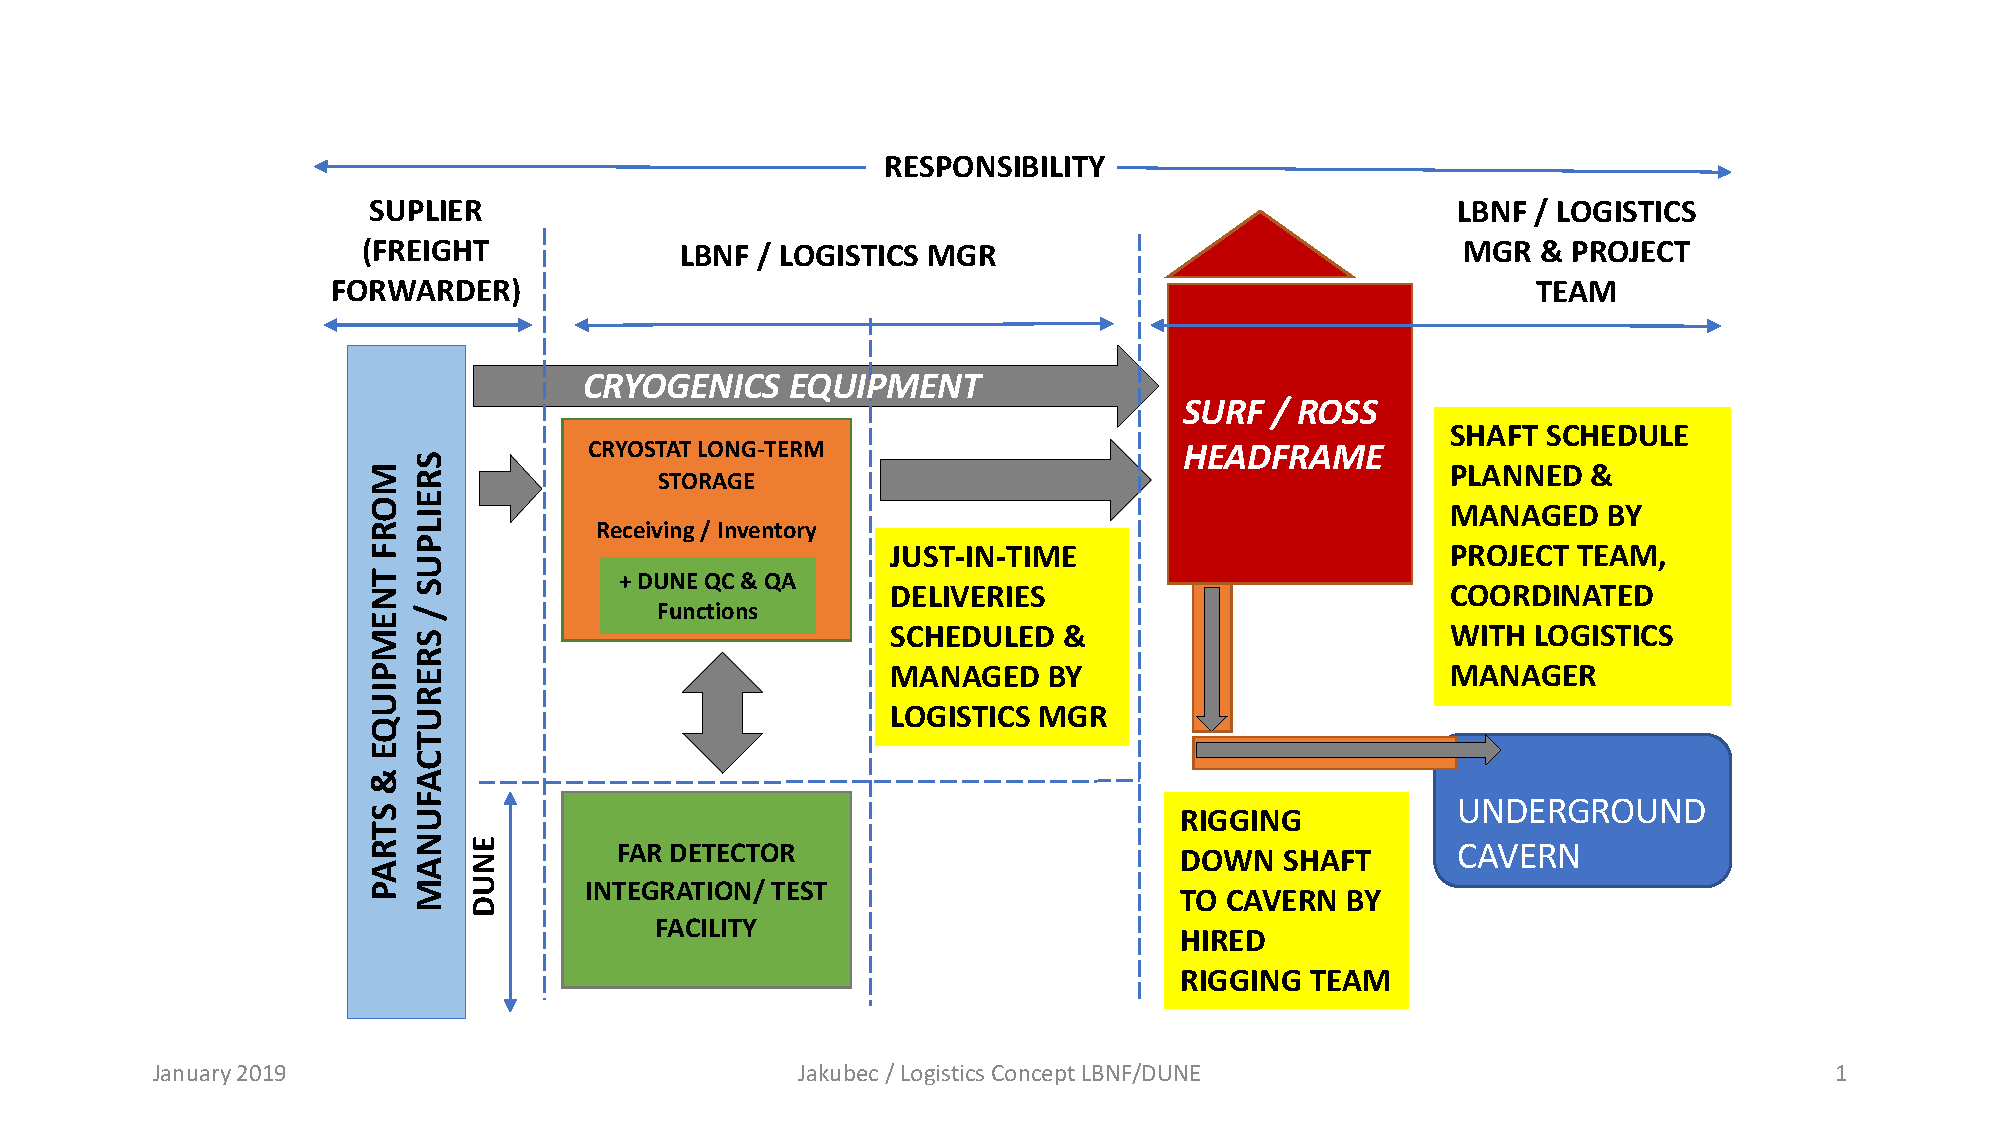
\includegraphics[width=\textwidth]{logistics-material-flow}
\end{dunefigure}

%%%%%%%%%%%%%%%%%%%%%%%%%%%%  
\subsection{Logistics Planning}
\label{sec:fdsp-tc-logPln}

The \dword{lbnf} and \dword{dune} logistics team oversees transportation of the cryostat (steel, foam, and membrane), the cryogenics system, the detector, and all related infrastructure not provided by the \dword{cf}. 
\dword{lbnf} specifically oversees the cryostat and cryogenics system, which are  discussed in detail in the \dword{lbnf} \dword{tdr}; because \dword{lbnf} material dominates the logistics, we present a summary.  
 \fixme{add ref to LBNF TDR when available}
The steel structure for each cryostat requires roughly 1,800 individual steel pieces,  some of which weigh up to \SI{7.5}{t}, as well as \SI{125}{t} of bolts to assemble the steel frame. 
The internal structure for each, which includes the foam insulation and the thin stainless steel membrane, requires transporting roughly 4,000 boxes, 
 each roughly 1.5 $\times$ 3.5 $\times$ 1.2 m$^3$. 
 The plan for cryostat installation, at present, calls for all components to be warehoused at the \dword{sdwf} before installation begins. 
This facility will need to have roughly $\SI{5,000}{m^2}$ of space available to the logistics operation approximately two years before installation of the first \dword{detmodule} begins. 
By the time detector components start arriving, most of the cryostat boxes will have been removed from the \dword{sdwf}, leaving ample space for the detector and the cryogenics components which are not delivered directly to the Ross Headframe. 
Additional space may be required if the boxes for the second cryostat arrive before  \dword{detmodule} \#1 installation is complete; a few buildings of the required size are available in the general area around \dword{surf}. 

\begin{dunefigure}
[Simplified model of the Ross Cage]
{fig:fdsp-tc-Cage}
{Simplified Ross Cage model and Specifications.}
\parbox{2.1in}{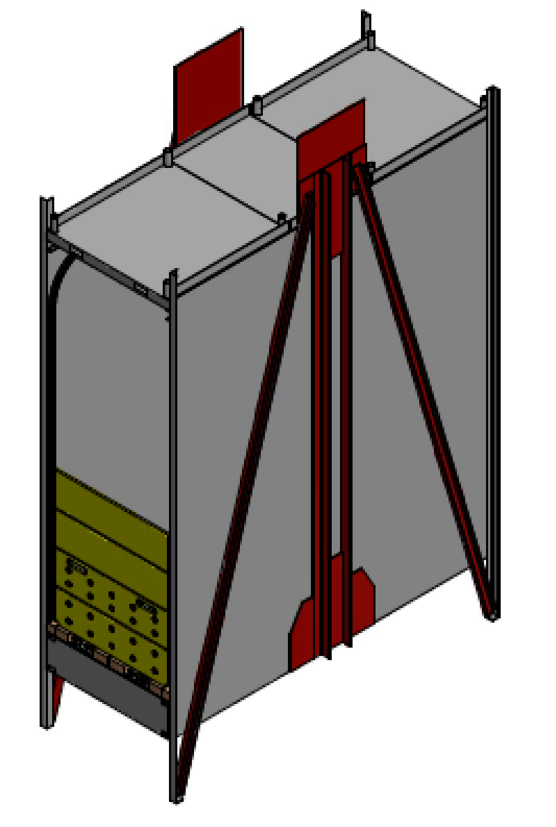
\includegraphics[width=0.3\textwidth]{graphics/Cage-view.pdf}}
\qquad\hspace{10pt}
\begin{minipage}{0.5\textwidth}%
\begin{tabular}{p{3.4cm}p{3.4cm}}        
\multicolumn{2}{c}{Ross Cage Specifications}\\ \toprowrule
Inside height & 3.6 m\\ \colhline
Inside depth  & 3.7 m \\ \colhline
Inside width  & 1.38 m \\ \colhline
Weight limit  &  5,897 kg \\ \colhline
Round trip \newline time & 17 min \newline (incl. unloading) \\ \colhline
\end{tabular}
\end{minipage}
\end{dunefigure}

The \dword{surf} Facility Access Specification~\cite{bib:docdb328} defines the limitations on dimensions and weights for all materials to be transported underground, the most stringent of which are set by the Ross shaft and cage. 
It is possible to bring material down the shaft underneath the cage or in the skip compartment  as a slung load, but this is a much slower process and requires careful planning, detailed procedures, and review. 
The \dword{dune} \dword{apa}s, for example, require this special handling because they are too tall to fit in the cage. 
Most material will be brought underground inside the cage. Figure \ref{fig:fdsp-tc-Cage} illustrates the new Ross cage and summarizes its parameters.  
The roundtrip travel time for the Ross cage is 17 minutes (actual travel time is \num{3.6} minutes each way), dominated by loading and unloading time.  
Slung loads will require more than an hour round trip.



The Ross Headframe has no loading dock so careful planning of material loading and unloading of shipments is required. 
All materials transported to it must arrive on a flatbed or curtain-sided chassis, where a forklift can unload  the items. 
The logistics team coordinates all deliveries from the \dword{sdwf} to the headframe, and the \dword{cf}-\dword{cmgc} coordinates all transport from there down the shaft.  
Most material will be delivered first to the \dword{sdwf}, where a central inventory system will capture data about the shipments.  
All deliveries, either from this warehouse or direct to the Ross Headframe, require (1) coordination with the logistics team, and (2) minimum two weeks prior notice, per an advance delivery plan.  
The logistics team will provide a shipping manual \cite{bib:docdb13954} to \dword{dune} institutions. 
It will specify guidelines for provision of shipping data and for cargo consignment such that the logistics team can monitor shipping progress and no delays occur due to incomplete or missing documentation. 


In \dword{pdsp}, delays in shipping and customs resulted in up to three weeks delay in the arrival of some parts, which necessitated significant re-planning of the installation work. 
To prevent this from becoming a much larger problem in \dword{dune}, we plan a minimum one month buffer of materials. 
This buffer will allow advance planning for the underground work, with confidence that all materials will be available as needed. 
Sufficient space must be made available in the warehouse and in the underground area  to house this material.
The \dword{sdwf} staff will de-consolidate or consolidate arriving cargo into appropriately sized boxes and crates, as needed, for delivery to \dword{surf}, to make the most efficient use of available trucks and the Ross Shaft. 

\begin{dunefigure}[Underground space needs during installation setup]{fig:fdsp-tc-setup}
  {CAD image showing the empty half of the north cavern as used during the installation setup phase of the first \dword{detmodule}.  Half of this empty space will be used for the cryostat work and half for storage of the detector infrastructure. The material shown outside the cavern must be stored in the \dword{sdwf}.}
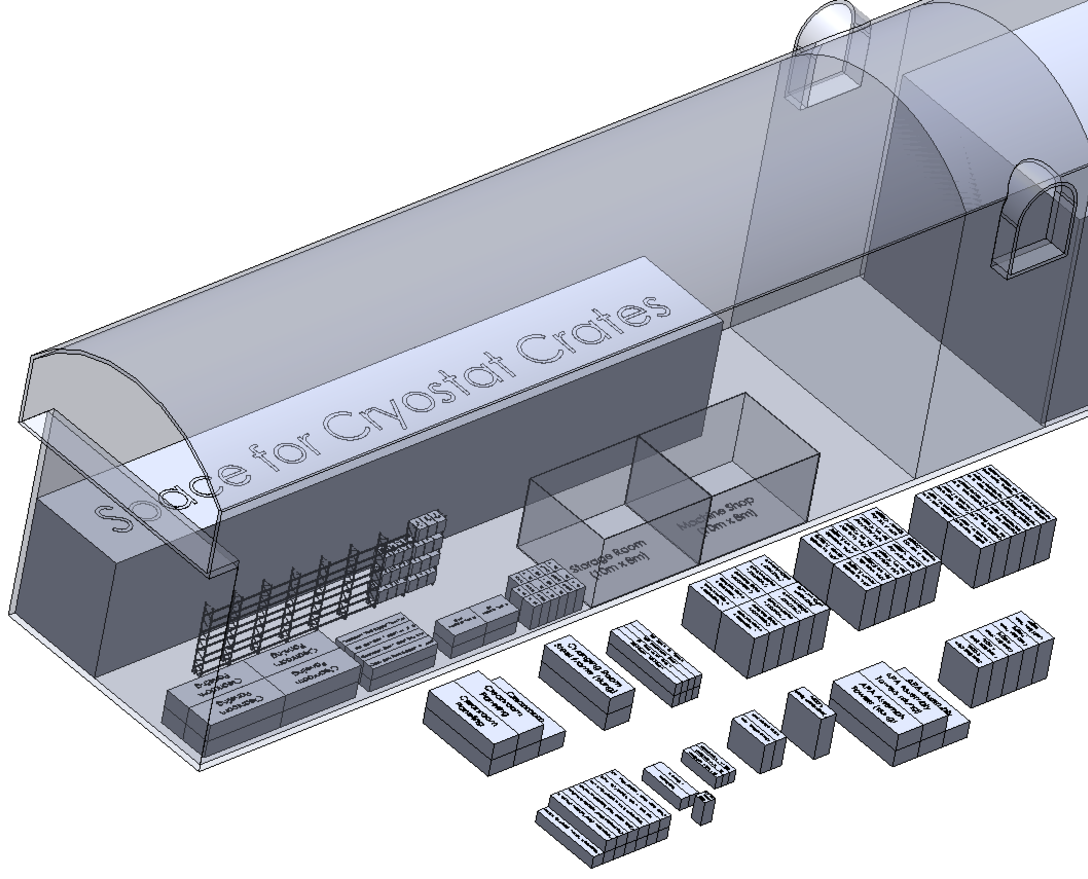
\includegraphics[width=.9\textwidth]{Material-Setup}
\end{dunefigure}


To determine the \dword{dune} storage space requirements and how much hoist time must be dedicated to \dword{dune}, a detailed inventory of all detector equipment and \dword{dune} infrastructure is needed. 
The complete list of the materials has been solicited from all consortia and technical coordination. 
The entries in the inventory spreadsheet are organized as \textquotedblleft loads\textquotedblright \ for the Ross shaft where a load is a crate or set of boxes that will be transported underground in one trip, either in the cage or as a slung load~\cite{bib:docdb8426}. 
Information captured in the load spreadsheet includes the number of  
trips, type of trip (slung load or cage), package dimensions, weight and type of package (crate, pallet, box, or carton). 

The load list at present predicts 1,600 hoist trips and approximately two  months of cage time, most of which is spread over one year. 
Detector installation (see Figure \ref{fig:high-level-schedule}) for the \dword{spmod} will span two years, so we divide the logistics planning into three phases: (1) the \dword{cuc} setup phase, (2) the installation setup phase, and (3) the detector installation phase. 
For each phase, a \threed model was generated to show how much material can be stored underground outside the work area and how much material must be stored on the surface. 
These models set the space requirements for the logistics on the surface. 
The phase with the largest amount of material to transport is the installation setup phase.  
Figure \ref{fig:fdsp-tc-setup} shows the model of the underground area and the required boxes for surface storage for the first third of the setup. 
This represents the first month of installation setup and shows that roughly 1,000 m$^2$ of warehouse space will be needed for \dword{dune} at this time.  The \dword{sdwf} will also need space to store up to 150 \dwords{apa}, 
adding 700 m$^2$ to the 1,000 m$^2$. 


%%%%%%%%%%%%%%%%%%%%%%%%%%%%
\subsection{Logistics Quality Control}
\label{sec:fdsp-tc-log-qaqc}


 
The \dword{protodune} experience offers a couple of significant lessons regarding logistics.

\begin{enumerate}
\item A central inventory system is essential for tracking  shipments.
\item It is important to avoid delays in shipping because they prevent installation work from  proceeding as planned. 
\end{enumerate}

The central inventory system  implemented at the \dword{sdwf}  and minimum one-month material buffer are the plans we have in place to prevent repetition of the schedule problems we experienced with \dword{pdsp}.   The full list of lessons learned from \dword{pdsp} is in~\cite{bib:docdb8255}. 

We do not foresee any component testing at the \dword{sdwf}, so the scope of the \dword{qc} work there is limited to two functions: 
The \dword{sdsd} logistics team in coordination with the facility will ensure that all materials fit in the Ross cage, or if a slung load is needed, that the necessary procedures are in place and approved before any material is transported to the Ross Headframe.  
The logistics provider will inventory all received shipments. DUNE representatives will verify that no obvious damage occurred in transport.

The contribution-in-kind model of this project complicates logistics oversight and inventory control as components will be delivered from many institutions and from different countries. 
Similarly the quality control information gathered during production and testing must be gathered from and accessible to all collaborators. 
Because of the complexity of the project and the different requirements for \dword{qc} and logistics oversight different data bases will be used for the two functions. A commercial \dword{wms} will control the inventory process at both the \dword{sdwf} (items both received and shipped) and at \dword{surf} (received at the Ross Headframe) while a separate data base the \dword{dcdb} will be used to store testing and other \dword{qc} data. The \dword{wms} will need to provide location and  \dword{qc} information to the \dword{dcdb} which will ultimately archive the construction data. The \dword{dcdb} has yet been designed.

Until materials arrive at the \dword{sdwf} or \dword{surf} (if directly shipped), the contributors' freight forwarding system will control the logistics supply chain, which will depend on the contractual circumstances and the contributor's choice. 
However, assuming the shipment is consigned as outlined in the 
shipping manual and the \dword{sdsd} logistics team therefore has access to the shipping data, this team will monitor the cargo progress and step in if a problem arises.
%However, the \dword{sdsd} logistics team will monitor the cargo progress and step in if a problem arises,  %since it will have access to the shipment data if 
%assuming the shipment is consigned as outlined in the %provided 
%shipping manual and the team has access to the shipping data. 
The \dword{sdwf} will be the ultimate point where the \dword{jpo} accepts %of capture for 
all the materials, except possibly for elements of the cryogenics system, given its special contractual requirements. The \dword{wms} will control basic receiving, inventory control, and shipping status for all components, parts, and equipment delivered to the \dword{sdwf}.
\fixme{Apr 10: See Anne's updates to the above pgraph, and a bit of rewording 4/11 after Ladia's re-edits}

The \dword{dcdb} will be the central repository for all \dword{qc} data. All relevant \dword{qc} data related to logistics must be transferred from the \dword{wms} to the \dword{dcdb} where it is archived. This information includes shipping reports and any reported damage. 
The \dword{qc} and shipping data flow is shown in Figure~\ref{fig:logistics-data-and-mat-flow}.

 


\begin{dunefigure}[QC and shipping data flow diagram for logistics ]{fig:logistics-data-and-mat-flow}
  {QC and shipping data flow diagram for the \dword{lbnf} and \dword{dune} logistics.}
 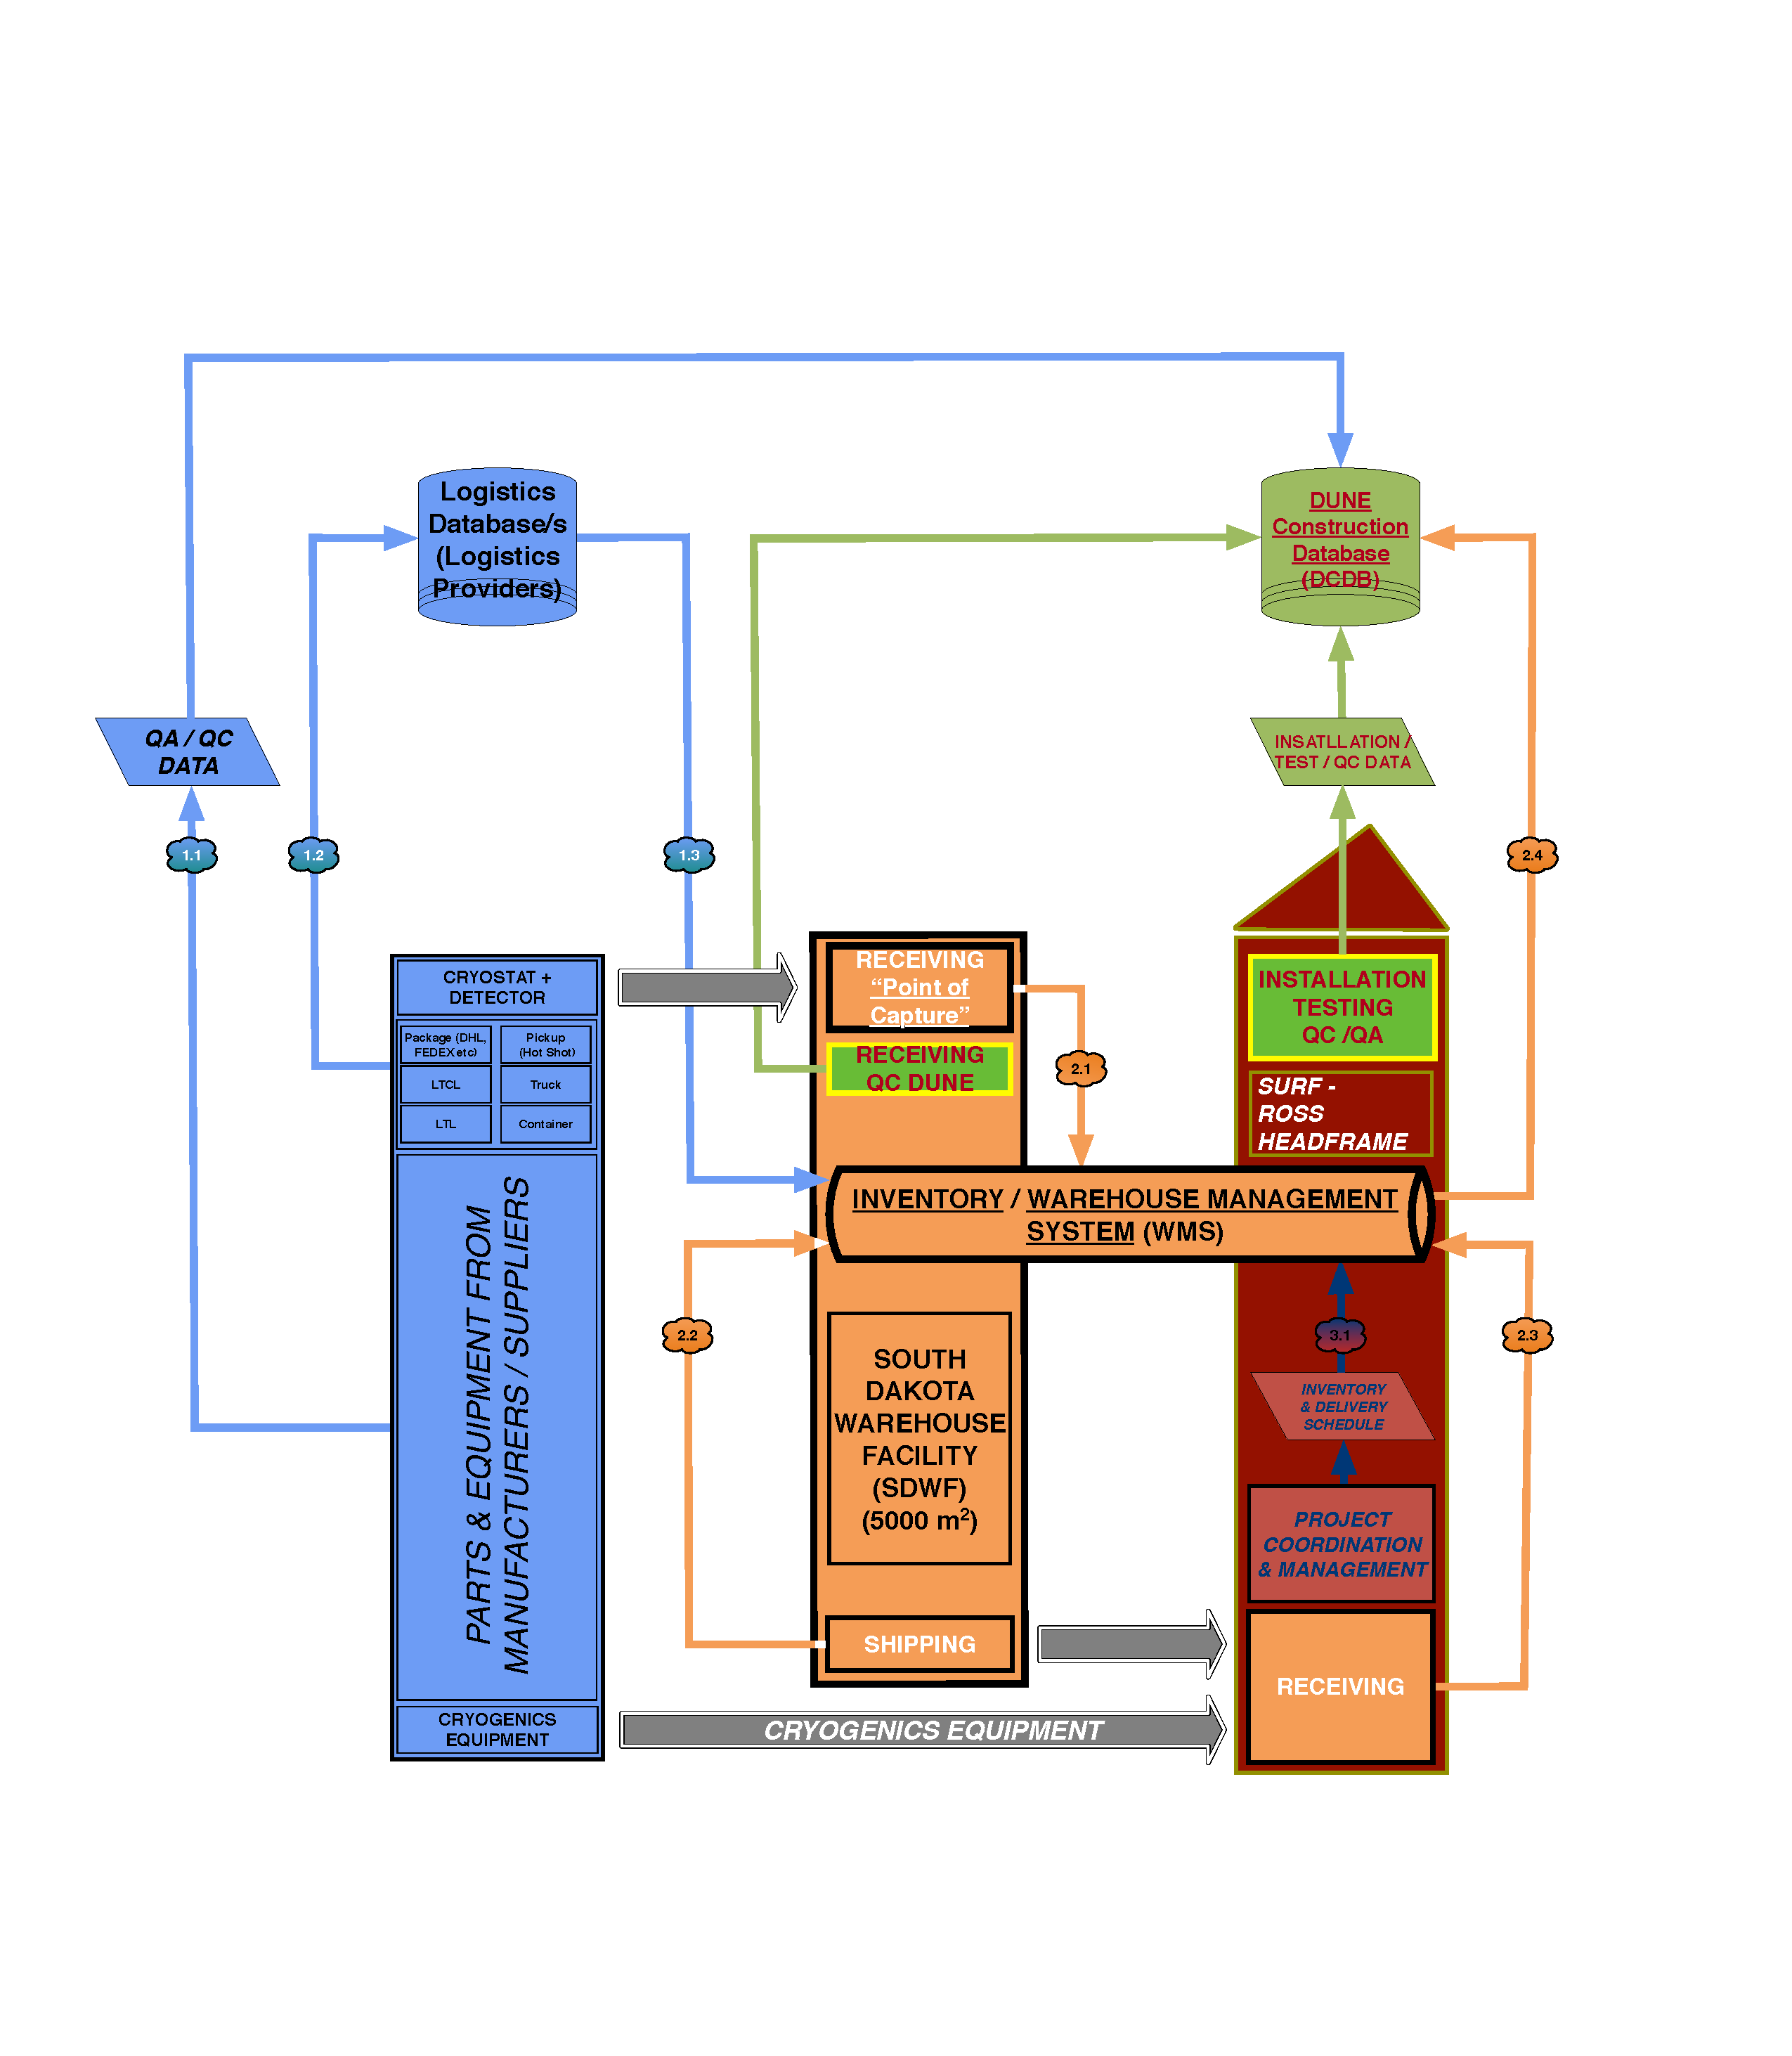
\includegraphics[width=\textwidth]{logistics-data-and-mat-flow}
\end{dunefigure}

 
The \dword{jpo} installation management team will provide a shipping (supply) report to the \dword{sdsd} logistics team and \dword{sdwf} for scheduling delivery of parts and equipment two weeks in advance of the required delivery date. 
All shipments will be inventoried upon receipt at the Ross Headframe in the \dword{wms}. 




%%%%%%%%%%%%%%%%%%%%%%%%%%%%
\subsection{Logistics Safety}
\label{sec:fdsp-tc-log-safety}

\fixme{talk with Mike A, Niehoff, Bill Miller}

%The \dword{lbnf}/\dword{dune} logistics facility is operated by \dword{sdsd}  as a Fermilab facility, but because of the international connections, we also follow CERN HSE, Fermilab ES\&H, and \dword{surf} ES\&H regulations.  Work is in progress to combine the three into a coherent list of codes and requirements. The \dword{dune} Project ES\&H Coordinator has overall ES\&H oversight responsibility for the \dword{dune} Project.  This person coordinates any activities and facilitates the resolution of any issues that cut across various divisions and institutions and subject to the requirements of the \dword{doe} Workers Safety and Health Program, Title 10, Code Federal Regulations (CRF) Part 851 (10 CFR 851). These requirements are promulgated through the Fermilab Directors Policy Manual and Fermilab ES\&H manual (FESHM), which align with the \dword{surf} ES\&H Manual.  Using the NOvA Far Detector Laboratory as a guideline for remote facilities, several other key documents guide the Logistics Center Safety Program.  The Building Safety Plan combines all building specific documents in a single folder:
The \dword{sdwf}  is operated by \dword{sdsd}  as a Fermilab facility, but because of the international collaboration, we  follow \dword{esh} regulations from CERN and \dword{surf} in addition to Fermilab's.  Work is in progress to combine the three into a coherent list of codes and requirements. The \dword{dune} Project \dword{esh} Coordinator has overall \dword{esh} oversight responsibility for the \dword{dune} Project.  This person coordinates any \dword{esh} activities and facilitates the resolution of any issues that are subject to the requirements of the \dword{doe} Workers Safety and Health Program, Title 10, Code Federal Regulations (CRF) Part 851 (10 CFR 851), and that cut across various divisions \fixme{divisions of what?} and institutions. These requirements are promulgated through the Fermilab Director's Policy Manual \fixme{ref} and Fermilab \dword{esh} manual (FESHM\cite{feshm}), which aligns with the \dword{surf} \dword{esh} manual.  Using the \dword{nova} Far Detector Laboratory as a guideline for remote facilities, several other key documents guide the Logistics Center Safety Program.  The Building Safety Plan \fixme{ref} combines all building specific documents in a single folder:

\begin{enumerate}
\item	Fire Safety and Building Emergency Evacuation Plan, which includes the fire evacuation plan, fire safety plan,  lockdown plans, and the site plan;
\item	Hazard Analysis document, which describes all typical hazards and their mediation %including 
procedures; 
\item	%SDS: 
Safety Data Sheets (SDS), 
\item	Respiratory Plan, as required for chemical or ODH hazards, and 
\item	Training Program, which covers required certifications and  training records.
\end{enumerate}

The current Technical Coordination Facilities Management Plan \fixme{ref} specifies a safety officer for the \dword{jpo} including the logistics facilities. This safety officer facilitates training, writes hazard analysis documents, runs weekly safety meetings, and keeps documentation records on materials-handling equipment and personnel information such as training, \dword{ppe} and other qualifications. 





